%%%%%%%%%%%%%%%%%%%%%%%%%%%%%%%%%%%%%%%%%%%%%%%%%%%%%%%%%%%%%%%
%
%     filename  = "YourName-Dissertation.tex",
%     version   = "1.3.0",
%     date      = "12/23/2014",
%     authors   = "Chris Dances,
%     copyright = "Chris Dances","Gary L. Gray"
%     address   = "Department of Mechanical and Nuclear Engineering
%                  137 Reber Bldg.,
%                  Penn State University,
%                  University Park, PA 16802,
%                  USA",
%     telephone = "916-524-8120",
%     email     = "chris.a.dances@gmail.com",
%
%%%%%%%%%%%%%%%%%%%%%%%%%%%%%%%%%%%%%%%%%%%%%%%%%%%%%%%%%%%%%%%
%
% Change History:
%
% 1.3.0	**	Added the cite package.
%
%		**	Give that the Graduate School now allows essentially
%			any line spacing, I have moved the line space setting
%			from psuthesis.cls to this driver file. Go ahead and
%			make it ugly if you want. :-)
%
%		**	Removed \addtocounter{page}{-1} after \psutitlepage is
%			executed. It made the paging of the frontmatter
%			incorrect. I can no longer remember why it was there.
%
%		**	Removed \psusigpage since the Graduate School now
%			provides the signature page.
%
%		**	Added the command \collegesubmittedto to add the College
%			in which the thesis/dissertation has been completed to
%			the title page.
%
%		**	Added instructions for documents that include a single
%			appendix since the Graduate School just hates calling it
%			``Appendix A'' is there is a single appendix.
%
%		**	Removed the fncychap package since I could not easily
%			find a way to make it work with documents that have a
%			single appendix.
%
%		**	Added the titlesec package so that the user can make the
%			format of the chapter titles a little less boring than
%			LaTeX's default.
%
% 1.2.2	**	Added some information to the main driver file (this
%			file) regarding the use of hyperref with the
%			psuthesis class. Thanks to Nathan Urban for pointing
%			out the included workaround.
%
% 1.2.1	**	Finally reproduced and fixed the problem where the
%			page number listed in the TOC for the Bibliography
%			was the last page number of the Bibliography.
%
%		**	Added 10pt and 11pt options to the document class,
%			though we have no idea why anyone would want to use
%			such insanely small font sizes since it will lead to
%			line lengths that are much too long.
%
% 1.2.0	**	Two additional class options have been added to
%			support honors theses submitted to the Schreyer
%			Honors College. These options are:
%			- honors
%			- honorsdepthead
%			See below for details.
%
%		**	We have also added the commands:
%			- honorsdegreeinfo
%			- honorsadviser
%			- honorsdepthead
%			Again, see below for details.
%
% 1.1.2	**	If you want to use the subfigure package with our
%			psuthesis class file, then you must must find the 
%			following line in the psuthesis.cls file:
%
%			\RequirePackage{tocloft}
%
%			and add the subfigure option. We have already set
%			this up for you in the psuthesis.cls file to make
%			this easy to do.
%
% 1.1.1	**	Added the fncychap package to the distribution.
%
% 1.1.0	**	The way that the thesis frontmatter and backmatter
%			is generated has been completely re-done in order
%			to be more intuitive.
%
%		**	We have added the ability to change the title of
%			the Dedication/Epigraph to anything you please.
%
%		**	In the process of changing the format of the Table
%			of Contents to conform to the inflexible rules of
%			the Grad School (the word ``Chapter'' and
%			``Appendix'' need to appear before the number and
%			letter, respectively), we have added an option to
%			the class called inlinechaptertoc that changes the
%			format of the Chapter/Appendix entries in the TOC.
%			Note that the tocloft package is now required.
%
%		**	Appendices should now start with the
%			\Appendix command rather than \chapter. See the
%			accompanying files for examples.
%
%		**	Added information regarding the Nontechnical
%			Abstract that is required of ESM students.
%
%		**	Added the fncychap package for those of you who like
%			the nice Chapter headings it provides. We like
%			Lenny, but you don't have to use it if you don't
%			want to. In addition, the other options are: Sonny,
%			Glenn, Conny, Rejne, and Bjarne
%
% 1.0.4	**	fixed the \addcontentsline entry for BibTeX within
%			the commented out text in the Bibliography section
%
% 1.0.3	**	added a sigpage option to conform to new Grad School
%			requirements
%
% 1.0.2	**	issued the \appendix command to start the appendices
%
%		**	moved the \addcontentsline for the bibliography so
%			that the bibliography now shows up on the right page
%			in the TOC
%
%		**	added some info if you use bibtex
%
% 1.0.1	**	eqlist and eqparbox are now included in the archive
%
%%%%%%%%%%%%%%%%%%%%%%%%%%%%%%%%%%%%%%%%%%%%%%%%%%%%%%%%%%%%%%%
%
% This is a template file to help get you started using the
% psuthesis.cls for theses and dissertations at Penn State
% University. You will, of course, need to put the
% psuthesis.cls file someplace that LaTeX will find it.
%
% We have set up a directory structure that we find to be clean
% and convenient. You can readjust it to suit your tastes. In
% fact, the structure used by our students is even a little
% more involved and commands are defined to point to the
% various directories.
%
% This document has been set up to be typeset using pdflatex.
% About the only thing you will need to change if typesetting
% using latex is the \DeclareGraphicsExtensions command.
%
% The psuthesis document class uses the same options as the
% book class. In addition, it requires that you have the
% ifthen, calc, setspace, and tocloft packages.
%
% The first additional option specifies the degree type. You
% can choose from:
%	Ph.D. using class option <phd>
%	M.S. using class option <ms>
%	M.Eng. using class option <meng>
%	M.A. using class option <ma>
%	B.S. using class option <bs>
%	B.A. using class option <ba>
%	Honors Baccalaureate using the option <honors>
%
% If you specify either ba or bs in addition to honors, it will
% just use the honors option and ignore the ba or bs option.
%
% The second additional option <inlinechaptertoc> determines
% the formatting of the Chapter entries in the Table of
% Contents. The default sets them as two-line entries (try it).
% If you want them as one-line entries, issue the
% inlinechaptertoc option.
%
% The class option ``honors'' should be used for theses
% submitted to the Schreyer Honors College. This option
% changes the formatting on the Title page so that the
% signatures appear on the Title page.
%
% The class option ``honorsdepthead'' adds the signature of the
% department head on the Title page for those baccalaureate
% theses that require this.
%
% The class option ``secondthesissupervisor'' should be used
% for baccalaureate honors degrees if you have a second
% Thesis Supervisor.
%
% The vita is only included with the phd option and it is
% placed at the end of the thesis. The permissions page is only
% included with the ms, meng, and ma options.
%%%%%%%%%%%%%%%%%%%%%%%%%%%%%%%%%%%%%%%%%%%%%%%%%%%%%%%%%%%%%%%
% Only one of the following lines should be used at a time.
%\documentclass[draft,phd,12pt]{psuthesis}
%\documentclass[draft,phd,inlinechaptertoc]{psuthesis}
%\documentclass[draft,ms]{psuthesis}
\documentclass[ms]{psuthesis}
%\documentclass[draft,honorsdepthead,honors]{psuthesis}
%\documentclass[phd,12pt]{psuthesis}
%\documentclass[draft,secondthesissupervisor,honors]{psuthesis}
%\documentclass[draft,bs]{psuthesis}

\usepackage[T1]{fontenc}
\usepackage{lmodern}
\usepackage{textcomp}
\usepackage{microtype}

%%%%%%%%%%%%%%%%%%%%%%%%%%%%
% Packages we like to use. %
%%%%%%%%%%%%%%%%%%%%%%%%%%%%
\usepackage{amsmath}
\usepackage{amssymb}
%\usepackage{amsthm}
%\usepackage{exscale}
%\usepackage[mathscr]{eucal}
%\usepackage{bm}
\usepackage{eqlist} % Makes for a nice list of symbols.
\usepackage[final]{graphicx}
\usepackage[dvipsnames]{color}
\DeclareGraphicsExtensions{.pdf, .jpg}

% http://www.tex.ac.uk/cgi-bin/texfaq2html?label=citesort
\usepackage{cite}

\usepackage{titlesec}

%%%%%%%%%%%%%%%%%%%%%%%%%%%%%%%
% Use of the hyperref package %
%%%%%%%%%%%%%%%%%%%%%%%%%%%%%%%
%
% This is optional and is included only for those students
% who want to use it.
%
% To the hyperref package, uncomment the following line:
\usepackage{hyperref}
%
% Note that you should also uncomment the following line:
\renewcommand{\theHchapter}{\thepart.\thechapter}
%
% to work around some a problem hyperref has with the fact
% the psuthesis class has unnumbered pages after which page
% counters are reset.

% Set the baselinestretch using the setspace package.
% The LaTeX Companion claims that a \baselinestretch of
% 1.24 gives one-and-a-half line spacing, which is allowed
% by the PSU thesis office. As of October 18, 2013, the Graduate
% School states ``The text of an eTD may be single-, double- or
% one- and-a-half-spaced.'' Go nuts!
\setstretch{1.24}


%%%%%%%%%%%%%%%%%%%%%%%%%%%%%%%%%%%%
% SPECIAL SYMBOLS AND NEW COMMANDS %
%%%%%%%%%%%%%%%%%%%%%%%%%%%%%%%%%%%%
% Place user-defined commands below.



%%%%%%%%%%%%%%%%%%%%%%%%%%%%%%%%%%%%%%%%%
% Renewed Float Parameters              %
% (Makes floats fit better on the page) %
%%%%%%%%%%%%%%%%%%%%%%%%%%%%%%%%%%%%%%%%%
\renewcommand{\floatpagefraction}{0.85}
\renewcommand{\topfraction}      {0.85}
\renewcommand{\bottomfraction}   {0.85}
\renewcommand{\textfraction}     {0.15}

% ----------------------------------------------------------- %

%%%%%%%%%%%%%%%%
% FRONT-MATTER %
%%%%%%%%%%%%%%%%
% Title
\title{INITIAL RESIDUAL FORMULATION of CTF}

% Author and Department
\author{Christopher A. Dances}
\dept{Nuclear Engineering}
% the degree will be conferred on this date
\degreedate{May 2015}
% year of your copyright
\copyrightyear{2015}

% This command is used for students submitting a thesis to the
% Schreyer Honors College. The argument of this command should
% contain every after the word ``requirements'' that appears on
% the title page. This provides the needed flexibility for
% all the degree types.
%\honorsdegreeinfo{for a masters degree \\ in Nuclear Engineering  \\ with a
% graudate minor in Computational Science}

% This is the document type. For example, this could also be:
%	Comprehensive Document
%	Thesis Proposal
\documenttype{Thesis}
%\documenttype{Dissertation}
%\documenttype{Comprehensive Document}


% This will generally be The Graduate School, though you can
% put anything in here to suit your needs.
\submittedto{The Graduate School}

% This is the college to in which you are submitting the
% thesis/dissertation.
\collegesubmittedto{College of Engineering}


%%%%%%%%%%%%%%%%%%
% Signatory Page %
%%%%%%%%%%%%%%%%%%
% You can have up to 7 committee members, i.e., one advisor
% and up to 6 readers.
%
% Begin by specifying the number of readers.
\numberofreaders{3}

% For baccalaureate honors degrees, enter the name of your
% honors adviser below.
%\honorsadviser{Honors P. Adviser}

% For baccalaureate honors degrees, if you have a second
% Thesis Supervisor, enter his or her name below.
%\secondthesissupervisor{Second T. Supervisor}

% For baccalaureate honors degrees, certain departments
% (e.g., Engineering Science and Mechanics) require the
% signature of the department head. In that case, enter the
% name of your department head below.
%\honorsdepthead{Department Q. Head}

% Input reader information below. The optional argument, which
% comes first, goes on the second line before the name.
\advisor[Thesis Advisor, Chair of Committee]
		{Maria Avramova}
		{Associate Professor of Nuclear Engineering}

\readerone[]
		{Kostadin Ivanov}
		{Distinghuished Professor of Nuclear Engineering}

\readertwo[Chair of Nuclear Engineering]
		{Arthur Motta}
		{Professor of Nuclear Engineering and Materias Science and Engineering}

\readerthree[Special Signatory]
		{Vince Mousseau}
		{Mentor from Sandia National Labs}


% Format the Chapter headings using the titlesec package.
% You can format section headings and the like here too.
\definecolor{gray75}{gray}{0.75}
\newcommand{\hsp}{\hspace{15pt}}
\titleformat{\chapter}[display]{\fontsize{30}{30}\selectfont\bfseries\sffamily}{Chapter \thechapter\hsp\textcolor{gray75}{\raisebox{3pt}{|}}}{0pt}{}{}

\titleformat{\section}[block]{\Large\bfseries\sffamily}{\thesection}{12pt}{}{}
\titleformat{\subsection}[block]{\large\bfseries\sffamily}{\thesubsection}{12pt}{}{}


% Makes use of LaTeX's include facility. Add as many chapters
% and appendices as you like.
\includeonly{%
Chapter-1/Chapter-1,Chapter-2/Chapter-2,Chapter-3/Chapter-3,Chapter-4/Chapter-4
%
}

\usepackage{listings}
%%%%%%%%%%%%%%%%%
% THE BEGINNING %
%%%%%%%%%%%%%%%%%
\begin{document}
%%%%%%%%%%%%%%%%%%%%%%%%
% Preliminary Material %
%%%%%%%%%%%%%%%%%%%%%%%%
% This command is needed to properly set up the frontmatter.
\frontmatter

%%%%%%%%%%%%%%%%%%%%%%%%%%%%%%%%%%%%%%%%%%%%%%%%%%%%%%%%%%%%%%
% IMPORTANT
%
% The following commands allow you to include all the
% frontmatter in your thesis. If you don't need one or more of
% these items, you can comment it out. Most of these items are
% actually required by the Grad School -- see the Thesis Guide
% for details regarding what is and what is not required for
% your particular degree.
%%%%%%%%%%%%%%%%%%%%%%%%%%%%%%%%%%%%%%%%%%%%%%%%%%%%%%%%%%%%%%
% !!! DO NOT CHANGE THE SEQUENCE OF THESE ITEMS !!!
%%%%%%%%%%%%%%%%%%%%%%%%%%%%%%%%%%%%%%%%%%%%%%%%%%%%%%%%%%%%%%

% Generates the title page based on info you have provided
% above.
\psutitlepage

% Generates the committee page -- this is bound with your
% thesis. If this is an baccalaureate honors thesis, then
% comment out this line.
\psucommitteepage

% Generates the abstract. The argument should point to the
% file containing your abstract. 
\thesisabstract{SupplementaryMaterial/Abstract}

% Generates the Table of Contents
\thesistableofcontents

% Generates the List of Figures
\thesislistoffigures

% Generates the List of Tables
\thesislistoftables

% Generates the List of Symbols. The argument should point to
% the file containing your List of Symbols. 
\thesislistofsymbols{SupplementaryMaterial/ListOfSymbols}

% Generates the Acknowledgments. The argument should point to
% the file containing your Acknowledgments. 
\thesisacknowledgments{SupplementaryMaterial/Acknowledgments}

% Generates the Epigraph/Dedication. The first argument should
% point to the file containing your Epigraph/Dedication and
% the second argument should be the title of this page. 
\thesisdedication{SupplementaryMaterial/Dedication}{Dedication}



%%%%%%%%%%%%%%%%%%%%%%%%%%%%%%%%%%%%%%%%%%%%%%%%%%%%%%
% This command is needed to get the main part of the %
% document going.                                    %
%%%%%%%%%%%%%%%%%%%%%%%%%%%%%%%%%%%%%%%%%%%%%%%%%%%%%%
\thesismainmatter

%%%%%%%%%%%%%%%%%%%%%%%%%%%%%%%%%%%%%%%%%%%%%%%%%%
% This is an AMS-LaTeX command to allow breaking %
% of displayed equations across pages. Note the  %
% closing the "}" just before the bibliography.  %
%%%%%%%%%%%%%%%%%%%%%%%%%%%%%%%%%%%%%%%%%%%%%%%%%%
\allowdisplaybreaks{
%\pagestyle{fancy}
%\fancyhead{}
%
%%%%%%%%%%%%%%%%%%%%%%
% THE ACTUAL CONTENT %
%%%%%%%%%%%%%%%%%%%%%%
% Chapters
%SourceDoc ../YourName-Dissertation.tex

\vspace*{-80mm}
\chapter{Introduction} \label{chapter1:introduction}

\pagenumbering{arabic}

For the past several decades, the primary focus in nuclear engineering within
the United States has been on light water reactors (LWR). Commercially,
all nuclear reactors are either boiling water reactors (BWR) or pressurized
water reactors (PWR). Correct computation of the thermal hydraulics within the
reactor core leads to efficient design and accuracy in the safety analysis. 
CASL is a key player in the effort, and through VERA \cite{Schmidt2014} utilizes
the popular subchannel code, CTF, for modeling the hydrodynamics within the reactor core.
This FORTRAN based code developed from COBRA-TF solves 8 conservation equations
for liquid, entrained droplet, and vapor phases phases, plus one conservation
equation for non-condensible gases \cite{CTF_theory}. The energy of the
entrained droplets is assumed to be in thermal equilibrium with the liquid
phase.

The set of procedures for ensuring that simulation codes such as CTF are
accurate and reliable is called software validation and verification
\cite{Oberkampf2008}. CTF has undergone software uncertainty quantification and
benchmark validation \cite{Avramova2015}. The current version of CTF has
standard verification practices that focus on software quality engineering
similar to those in other versions of COBRA-TF \cite{Aumiller2013}, but
currently lacks an in depth verification document that focuses on numerical
algorithm verification. This work focuses on this second type of verification
for the original version of CTF as well as a residual formulation. 

The 1-D residual formulation of the code has been created for single phase
liquid coupled to radial conduction. While other residual formulations have been
formed for other versions of COBRA-TF \cite{Lloyd2014}, none have been
integrated into the CASL version of CTF. This work details the verification of
both the residual formulation and the original version of CTF for the single
phase liquid and radial conduction equations. The verification problems will
study of the order of accuracy of the errors, which is considered one of the
more rigorous verification criteria \cite{Roy2005}. This work will be
considered a starting point for future work to perform verification on the
single phase equations in both axial and transverse dimensions
\cite{Merroun2009}, and two phase flow \cite{Mahadevan2009}.

%\section{CTF}
%SourceDoc ../YourName-Dissertation.tex
\vspace*{-80mm}
\chapter{Conservation Equations} \label{chapter2:conservation_equations}
	
	
\section{Single Phase Liquid Euler Equations} \label{sec:euler_equations}
	
	The finite volume structure in CTF in figure \ref{fig:CTF-Cells} is for
	a one-dimmensional channel in the axial direction with $n$ number of cells.
	The first and last cells at $0$ and $n+1$ are ghost cells and act as the
	boundary conditions for the problem. Pressure, enthalpy, and density are
	averaged over the cell volume and are located at the center of the cell.
	Velocity is located at the faces in between cells and averaged over the flow
	area of the surface. The cells are represented with an index $i$, and the
	faces with indexes of $i+\frac{1}{2}$ or $i-\frac{1}{2}$. This project will
	initially focus on this 1-D configuration. Usually the code is three
	dimensional, with channels connecting to each other in two more dimensions.
	Fully 3-D equations will be considered in future work.
	
	\begin{figure}[!h]
		\centering
		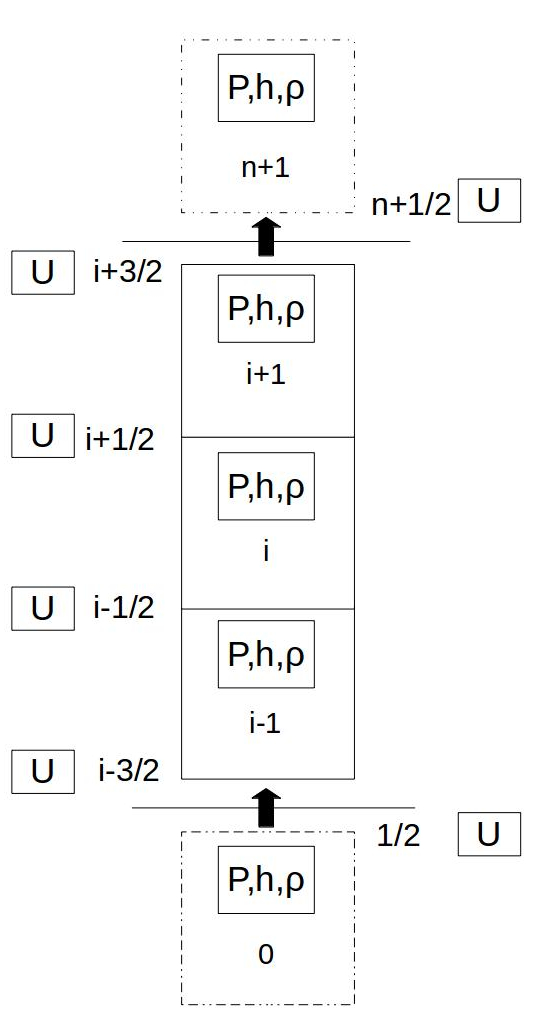
\includegraphics[width=0.30\textwidth]{images/CTF-Cells}
		\caption{The finite volume structure for CTF}
		\label{fig:CTF-Cells}
	\end{figure}

	The thermal hydraulics of a LWR core is an important part of nuclear
	reactor design. CTF solves 8 conservation equations for liquid,
	entrained droplet, and vapor phases of water boiling within the rod structure
	of a LWR reactor core \cite{Salko2014}. Currently, the discretized conservation
	equations are analytically reduced into a pressure matrix. This pressure
	matrix is then solved for using a semi-implicit method and the new time
	fluid quantities are back calculated using the new time pressure values. The
	rod temperatures are implicitly solved for using an explicit coupling with the
	fluid solution.  This work involves representing the 1-D single phase liquid
	conservation equations and calculated variables in a residual formulation. The
	full Jacobian matrix can then be built numerically, and  can then either be
	reduced to a pressure matrix or solved directly. Verification of the residuals
	was done by comparing calculated results to analytical solutions for isokinetic
	advection and shock tube problems. For each verification problem, a scaling
	study of the truncation error was compared to the predicted behavior derived
	from modified equation analysis using Richardson extrapolation. Further work
	was then applied to represent 1-D heat conduction within nuclear rod types.
	The fluid solution can be solved for semi-implicitly, or implicitly with either
	explicit or implicit coupling to the solid implicit solution . The single phase
	Euler partial differential equations for mass \eqref{eq:pde_mass}, momentum
	\eqref{eq:pde_momentum}, and energy \eqref{eq:pde_energy} correspond to the
	unknown variables pressure $P$, velocity $u$, and enthalpy $h$. The equation
	of state \eqref{eq:pde_EOS} realates density $\rho$ as a function of pressure
	and enthalpy. The first terms in each of the equations are temporal terms. The
	rest of the terms are steady state spatial terms. The last term in the energy
	equation represents the net heat transfer from the adjacent rods to the
	current fluid subchannel.
    
    \begin{equation}
    	\label{eq:pde_mass}
    	\frac{ \partial \rho}{\partial t} + \bigtriangledown \rho u = 0
    \end{equation}
    
    \begin{equation}
    	\label{eq:pde_momentum}
    	\frac{ \partial \rho u}{\partial t} + \bigtriangledown \rho u^{2} +
    	\bigtriangledown P - \rho g  = 0
    \end{equation}
    
    \begin{equation}
    	\label{eq:pde_energy}
    	\frac{ \partial \rho h}{\partial t} -
    	\frac{ \partial  P}{\partial t} + 
    	\bigtriangledown ( \rho  u h )%  -
    	+ \frac{q_{rod}}{\forall_{fluid}}
    	= 0
    \end{equation}
    
    \begin{equation}
    	\label{eq:pde_EOS}
    	\rho = EOS(P,h)
    \end{equation}
    
    The 1-D formulation of the Euler Equations will assume a direction $x$ as shown
    in the 1-D mass equation \eqref{eq:1-D_mass}. The momentum and energy equations
    are represented in a non-conservative form as shown in equations
    \eqref{eq:1-D_momentum_long} and \eqref{eq:1-D_energy_long}. The momentum
    equation contains a term that has a product of the left hand side of the 1-D
    mass equation. This terms can therefore be dropped since it is equivalent
    to zero, and the entire equation can be divided by density to give a simpler
    form of the momentum equation \eqref{eq:1-D_momentum}. The last term in the
    energy equation represents the net heat transfer from the adjacent rods to
    the current fluid subchannel. This is equated as the surface area of
    the rod liquid interface times the heat transfer coefficient and temperature
    difference between the wall and bulk fluid temperatures. 
    
    \begin{equation}
    	\label{eq:1-D_mass}
    	\dfrac{ \partial \rho }{ \partial t} +
    	\dfrac{ \partial \rho u}{\partial x} = 0
    \end{equation}
    
    \begin{equation}
    	\label{eq:1-D_momentum_long}
    	\rho \dfrac{ \partial u }{ \partial t } + 
    	u \left(  \dfrac{ \partial \rho }{ \partial t } +
    	          \dfrac{ \partial \rho u }{\partial x} \right) +
    	\rho u \dfrac{ \partial u}{ \partial x} + 
    	\dfrac{ \partial P}{ \partial x}   - \rho g
    	= 0
    \end{equation}
    
    \begin{equation}
    	\label{eq:1-D_momentum}
    	\dfrac{ \partial u }{ \partial t } + 
    	u \dfrac{ \partial u }{ \partial x } + 
    	\dfrac{1}{ \rho } \dfrac{ \partial P }{ \partial x } - g  
    	= 0
    \end{equation}
    
    \begin{equation}
    	\label{eq:1-D_energy_long}
    	\rho \frac{ \partial  h}{\partial t} -
    	     \frac{ \partial  P}{\partial t} + 
    	h    \frac{ \partial  \rho}{\partial t} +
    	\rho u \frac{ \partial h }{ \partial x} +
    	h    \frac{ \partial \rho u }{ \partial x} 
    	+ \frac{2\pi r_{rod}}{A_{i}}h_{l}\left(T_{wall}-T_{fluid}\right)
    	= 0
    \end{equation}
    
    The 1-D equations are then evaluated at a position index $ i $ and a certain
    time $n$ in order to solve for the next time value of $n+1$. In the mass equation
    \eqref{eq:FD_mass}, the velocities are located at the cell faces
    $i+\frac{1}{2}$ and $i-\frac{1}{2}$. The density  in the mass and energy
    equations is upwinded $\dot{\rho}_{i+\frac{1}{2}}^{n}$ and averaged
    $\bar{\rho}_{i+\frac{1}{2}}^{n}$ in the momentum equation. In equation
    \eqref{eq:FD_momentum}, the derivative $\frac{ \partial u}{ \partial x}$ is
    upwinded assuming that the flow is positive. In the energy equation,
    \eqref{eq:FD_energy} the enthalpy values in the first spatial term are
    upwinded and shown here assuming a positive velocity. The equation of state
    \eqref{eq:EOS} solves for density assuming that it is a linear combination
    of changes due to pressure and enthalpy. The partial derivatives in the
    equation are calculated from steam tables as functions of old time pressure
    and enthalpy.
    
    \begin{equation}
    	\label{eq:FD_mass}
    	\frac{ \rho_{i}^{n+1}-\rho_{i}^{n}}{ \Delta t} +
    	\frac{ \dot{\rho}_{i+\frac{1}{2}}^{n} u_{i+\frac{1}{2}}^{n+1}  -
    	\dot{\rho}_{i-\frac{1}{2}}^{n}  u_{i-\frac{1}{2}}^{n+1} }{\Delta x}
    	 = 0
    \end{equation}
    
    \begin{equation}
    	\label{eq:FD_momentum}
    	\frac{  u_{i+\frac{1}{2}}^{n+1} - u_{i+\frac{1}{2}}^{n} }{ \Delta t } + 
    	u_{i+\frac{1}{2}}^{n} \left( \frac{  u_{i+\frac{1}{2}}^{n} -
    	u_{i-\frac{1}{2}}^{n}}{ \Delta x} \right) +
    	\frac{1}{\bar{\rho}_{i+\frac{1}{2}}^{n} } 
    	\frac{ P_{i+1}^{n+1} -P_{i}^{n+1} }{ \Delta x } - g
    	= 0
    \end{equation}
    
    \begin{multline}
    	\label{eq:FD_energy}
    	\rho_{i}^{n} \frac{ h_{i}^{n+1} - h_{i}^{n}}{\Delta t} 
    	+ h_{i}^{n} \frac{ \rho_{i}^{n+1} - \rho_{i}^{n}}{\Delta t} 
    	- \frac{P_{i}^{n+1}-P_{i}^{n}}{\Delta t}
    	+ \left( \rho u \right)_{i}^{n} 
    		\frac{   h _{i}^{n}  - h _{i-1}^{n} }{\Delta x}  \\
    	+ h _{i}^{n} \frac{ \dot{\rho}_{i+\frac{1}{2}}^{n} u_{i+\frac{1}{2}}^{n+1} 
    	- \dot{\rho}_{i-\frac{1}{2}}^{n}  u_{i-\frac{1}{2}}^{n+1} }{\Delta x}
    	+ \frac{2\pi r_{rod}}{A_{i}}h_{l}\left(T_{wall}-T_{fluid}\right)
    	= 0
    \end{multline}
    
    \begin{equation}
    	\label{eq:EOS}
    	\rho_{i}^{n+1} - \rho_{i}^{n} = 
    	\left( \frac{ \partial \rho }{\partial P} \bigg|_{i}^{n}  \right) 
    	\left( P_{i}^{n+1} - P_{i}^{n} \right)
    	+ 
    	\left( \frac{ \partial \rho }{\partial h} \bigg|_{i}^{n} \right)
    	\left( h_{i}^{n+1} - h_{i}^{n} \right)
    \end{equation}

\section{1-D Radial Solid Conduction Equation} \label{sec:rad_conduction}

The conduction equation for a cylindrical system is given in equation \ref{eq:full_conduction}.
The first  term represents the amount of energy stored within the solid area within
a unit  time. The second term is the conduction in the radial direction. The
second  and third terms are the conduction in the azimuthal and axial
directions,  respectively. The last term represents the heat generation within
the solid.

\begin{equation}
	\label{eq:full_conduction}
	  \rho_{fuel}c_{p}\frac{\partial T}{\partial t}
	- \frac{1}{r}\frac{\partial}{\partial r}\left( 
		kr\frac{\partial T}{\partial r}\right)
	- \frac{1}{r^{2}}\frac{\partial}{\partial \theta}\left(
		k\frac{\partial T}{\partial \theta}\right)
	- \frac{\partial}{\partial z}\left(k\frac{\partial T}{\partial z}\right) 
	- q'''
	= 0
\end{equation}

This work focuses on the 1D radial equations setting the derivatives with
respect to the angular and axial directions to zero. Equation \ref{eq:full_conduction} now reduces
to equation \ref{eq:rad_conduction}.

\begin{equation}
	\label{eq:rad_conduction}
	  \rho_{fuel}c_{p}\frac{\partial T}{\partial t}
	- \frac{1}{r}\frac{\partial}{\partial r}\left( 
		kr\frac{\partial T}{\partial r}\right)
	- q'''
	= 0
\end{equation}

When the radius is zero, the fuel temperature is considered to be a maximum
giving the boundary condition in equation \ref{eq:bc_centerline}

\begin{equation}
	\label{eq:bc_centerline}
	\left(\frac{\partial T}{\partial r}\right)_{r=0}=0
\end{equation}

\begin{figure}[!h]
	\centering
	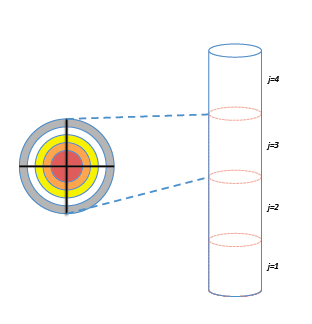
\includegraphics[width=0.40\textwidth]{images/rod-axial.png}
	\caption{Rod Axial Mesh}
	\label{fig:rod-axial}
\end{figure}

The nuclear rod geometry types in CTF are meshed at each axial level according
to figure \ref{fig:rod-axial}. Each axial level will be meshed as seen in figure
\ref{fig:radial_diagram} where the red region is fuel and the grey region is
cladding. The black dots represent the nodes within the fuel. Each node covers
a region within the rod as bounded by the dashed lines. The nodes within the
fuel are located at the center of the region. Each region is assumed to have
uniform properties with values evaluated at the node. The last node within  the
fuel is located at the surface of the fuel at the interface with the gap. 
There are two additional nodes that represent the outer clad surface and the
inner  clad surface respectively. The gap between the outer surface of the fuel
and the inner surface of the cladding has a specified heat transfer coefficient
or is calculated using the dynamic gap conductance model.

	\begin{figure}[!h]
		\centering
		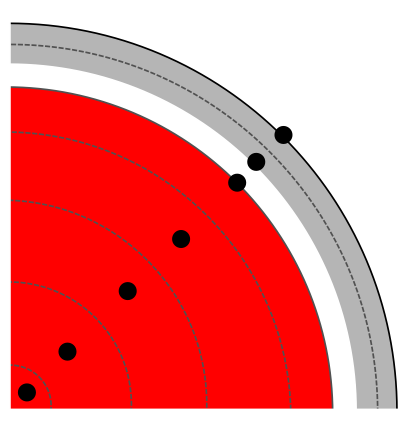
\includegraphics[width=0.40\textwidth]{images/radial_diagram.png}
		\caption{Radial Rod Meshing}
		\label{fig:radial_diagram}
	\end{figure}
	
The outer surface of the cladding is assumed to be in contact with the fluid in
the  adjacent channel on that axial level. The rods have the same number of
axial  levels as the fluid, but do not have ghost cells at the top and bottom.
Instead  the first and last fluid axial levels are connected to two rod axial
levels as  shown by Figure \ref{fig:fluid-solid-meshing}, where the rod axial
levels are on the left, and the fluid  axial levels are on the right. The light
blue cells are the fluid ghost cells.

	\begin{figure}[!h]
		\centering
		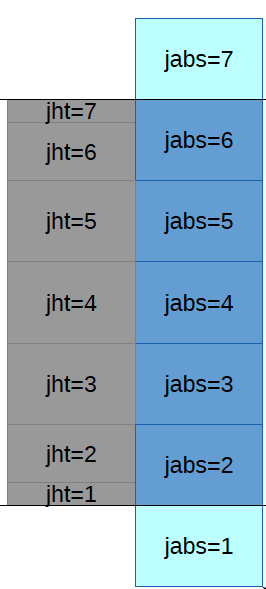
\includegraphics[width=0.20\textwidth]{images/fluid-solid-meshing.png}
		\caption{Radial Rod Meshing}
		\label{fig:fluid-solid-meshing}
	\end{figure}

The conduction equation can be approximated using the finite difference method,
or the control volume difference method \cite{Botte2000}. The control volume
method will be used  since it is the same method utilized in the original
version of CTF. The implicit  finite difference equation now looks like equation
\ref{eq:rod:fuel:conduction}.

\begin{equation}
	\small
	\label{eq:rod:fuel:conduction}
	  \rho_{fuel}c_{p,i}\frac{T^{n+1}_{i}-T^{n}_{i}}{\Delta t}
	- \frac{2\pi}{A_{i}}\left( 
		\left(k_{i+\frac{1}{2}}r_{i+\frac{1}{2}}
		\frac{T^{n+1}_{i+1}-T^{n+1}_{i}}{\Delta r_{i+\frac{1}{2}}}\right)
 	  - \left(k_{i-\frac{1}{2}}r_{i-\frac{1}{2}}
		\frac{T^{n+1}_{i}-T^{n+1}_{i-1}}{\Delta r_{i-\frac{1}{2}}}\right)
	  \right)
	- q_{i}'''
	= 0
\end{equation}

The density on the temporal term is defined as the cold mass of the node divided
by the volume of the node. The temporal derivative is approximated with first
order accurate forward differencing. The spatial derivatives are evaluated at the right
boundary, $i+\frac{1}{2}$, and at the left boundary,$i-\frac{1}{2}$ using first
order forward differencing. When $i=1$ at the inner most node, the radius at the
left boundary and the derivative of the temperature is zero. At the boundary
between the surface of the fuel and the inside surface of the cladding, a
different set of finite difference equations are needed as given by equation
\ref{eq:rod:fuel_surface:conduction}

\begin{equation}
	\label{eq:rod:fuel_surface:conduction}
	  \rho_{fuel}c_{p,i}\frac{T^{n+1}_{i}-T^{n}_{i}}{\Delta t}
	+ \frac{2\pi}{A_{i}}
 	    \left(k_{i-\frac{1}{2}}r_{i-\frac{1}{2}}
		\frac{T^{n+1}_{i}-T^{n+1}_{i-1}}{\Delta r_{i-\frac{1}{2}}}\right)
	- \frac{2\pi r_{i}h_{gap}}{A_{i}}\left(T^{n+1}_{i+1}-T^{n+1}_{i}\right)
	- q_{i}'''
	= 0
\end{equation}

The finite difference equation between the inner and outer cladding surfaces
given by equation \ref{eq:rod:clad_inner:conduction} has no heat generation or
conduction from the fuel. Instead the  volumetric heat rate is calculated using
the term for the volumetric heat rate  across the gap and a similar term but for
the volumetric heat rate across the cladding. Since the cladding does not have
any heat generation, this  term is represented as the temperature difference
across the cladding times the thermal resistance across the cladding  times the
perimeter of the cladding divided by the area of the inner cladding region.

\begin{equation}
	\label{eq:rod:clad_inner:conduction}
	  \rho_{clad}c_{p,i}\frac{T^{n+1}_{i}-T^{n}_{i}}{\Delta t}
	+ \frac{2\pi r_{i}h_{gap}}{A_{i}}\left(T^{n+1}_{i}-T^{n+1}_{i-1}\right)
	- \frac{2\pi}{A_{i}}
 	    \left(k_{i+\frac{1}{2}}r_{i+\frac{1}{2}}
		\frac{T^{n+1}_{i+1}-T^{n+1}_{i}}{\Delta r_{i+\frac{1}{2}}}\right)
	= 0
\end{equation}

The finite difference equation between the inner and outer cladding surfaces
given by equation \ref{eq:rod:clad_outer:conduction} relates the wall
temperature to the bulk fluid temperature at the same axial level. The
volumetric heat rate lost to the fluid is represented as the temperature
difference between the wall and the fluid times the thermal resistance of the
fluid and divided by the outer cladding region.

\begin{equation}
	\label{eq:rod:clad_outer:conduction}
	  \rho_{clad}c_{p,i}\frac{T^{n+1}_{i}-T^{n}_{i}}{\Delta t}
	+ \frac{2\pi}{A_{i}}
 	    \left(k_{i-\frac{1}{2}}r_{i-\frac{1}{2}}
		\frac{T^{n+1}_{i}-T^{n+1}_{i-1}}{\Delta r_{i-\frac{1}{2}}}\right)
    - \frac{2\pi r_{i}h_{fluid}}{A_{i}}\left(T^{n+1}_{i}-T^{k}_{fluid}\right)
	= 0
\end{equation}

The numerator in the last term is also in the fluid energy conservation
equation. The heat transfer coefficient is currently calculated using the
Dittus-Boelter correlation \cite{Incropera1998}. The fluid properties are
evaluated at the bulk fluid temperature. When the fluid finite equations are
solved for implicitly, they will impact the solid conduction equations through
the calculation of the heat transfer coefficient and the fluid temperature.
%SourceDoc ../YourName-Dissertation.tex
\vspace*{-80mm}
\chapter{Residual Formulation and Jacobian Construction}
\label{chapter3:residual_formulation}
	    
    A residual is simply the difference between the value at some future time
    $n+1$ and the value at the current iteration $k$. This can be applied to
    desired variables as shown in equations %Source?
    \eqref{eq:residual_def:P}, \eqref{eq:residual_def:h},
    \eqref{eq:residual_def:u}, and \eqref{eq:residual_def:rho}. Residuals can
    also be applied to the conservation equations by substituting the definition
    of the residual variables into the conservation equations. This will
    effectively change any variables evaluated at $n+1$ to $k$. Each cell will
    have three residual variables and three residual equations. For the entire
    solution, we will then have a residual variable array $\delta X$, and a
    residual function array $F(X)$ which defines a linear system as seen in 
    equation \eqref{eq:linear_system}.
        
    \begin{equation}
    	\label{eq:residual_def:P}
    	\delta P_{i} = P^{n+1}_{i} - P^{k}_{i}
    \end{equation}
    
    \begin{equation}
    	\label{eq:residual_def:h}
    	\delta h_{i} = h^{n+1}_{i} - h^{k}_{i}
    \end{equation}
    
    \begin{equation}
    	\label{eq:residual_def:u}
    	\delta u_{i+\frac{1}{2}} = u^{n+1}_{i+\frac{1}{2}} - u^{k}_{i+\frac{1}{2}}
    \end{equation}
    
    \begin{equation}
    	\label{eq:residual_def:rho}
    	\delta \rho_{i} = \rho^{n+1}_{i} - \rho^{k}_{i}
    \end{equation}
    
    \begin{equation}
    	\label{eq:linear_system}
    	J \delta X = - F(X)
    \end{equation}
    
    The Jacobian matrix is defined in equation \eqref{eq:jac_def} as the derivative
    of each response of the function $F_{j}$ with respect to each variable $X_{i}$.
    The derivative can be calculated numerically as shown by equation
    \eqref{eq:jac_numerical} where $\epsilon$ is a small numerical value. For
    COBRA-TF the equations are linear, and this numerical approximation
    of the Jacobian matrix is exact. This should produce the same jacobian
    matrix that COBRA-TF currently generates analytically. 
    
    \begin{equation}
    	\label{eq:jac_def}
    	J_{i,j}=\frac{ \partial F_{j}(X)}{\partial X_{i}}
    \end{equation}
    
    \begin{equation}
    	\label{eq:jac_numerical}
    	J_{i,j}  \approx \frac{F_{j}(X_{i}+\epsilon)-F_{j}(X)}{\epsilon}
    \end{equation}
    
    To build the jacobian matrix, an object oriented class was created that
    contains three arrays. An array that points to the residual functions, an
    array that points to the position within a target variable arrray, and an
    array that has the index that the function is to be evaluated at. These
    lists can be appended to in any order, but have to be appended all at the
    same time so that variables and functions must correspond with each other.
    Then to construct the jacobian matrix, the residual function and residual
    variable arrays can each be looped over to numerically build the jacobian
    matrix as seen in figure \ref{fig:Jacobian_Setup}. 
    
    \begin{figure}[!h]
    	\centering
    	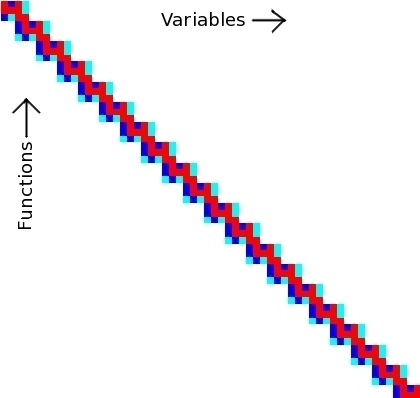
\includegraphics[width=0.35\textwidth]{images/Jacobian_Setup}
    	\caption{Strucutre of the jacobian matrix for single phase liquid}
    	\label{fig:Jacobian_Setup}
    \end{figure}


	The explicitly coupled solid liquid Jacobian matrix can be seen in figure
	\ref{fig:Explicit-Diagram}, where blue values represent negative entries and
	red values positive entries. The black lines were drawn on top of the image to
	represent artificial boundaries between the liquid Jacobian matrix in the top
	left corner and the solid Jacobian matrix in the top right corner. The fluid
	Jacobian matrix contains 3 conservation equations for every axial level. The
	liquid function residuals are appended in the order of mass conservation,
	energy conservation, and momentum conservation for each axial level. These
	correspond the pressure, enthalpy, and velocity at each axial level. The liquid
	Jacobian matrix can be evaluated as either semi-implicit or fully implicit. The
	solid Jacobian matrix contains 1 energy conservation equation for each node in
	the rod. Since axial and azimuthal conduction are not computed, each radial
	level is computed separately from the rest. This can be seen by the lack of
	cross terms in the Jacobian matrix at each axial level. The Jacobian matrix on
	the right is an implicit coupling between the implicit liquid Jacobian matrix
	and the implicit solid matrix. The cross terms in the top right corner
	represent the effect of the wall temperature on the energy equation in the
	liquid Jacobian matrix. The terms on the bottom left represent the effects of
	pressure, enthalpy, and velocity on the energy equation in the solid Jacobian
	matrix. The implicit matrix is unconditionally stable, allowing for time steps
	greater than the material Courant limits. Once the coupled Jacobian matrix is
	constructed, it is solved using the linear Krylov solver from PETSC . The
	residuals for each of the conservation equations are then L2 normalized over
	the domain to determine the convergence of the system.
	
	\begin{figure}[!h]
    	\centering
    	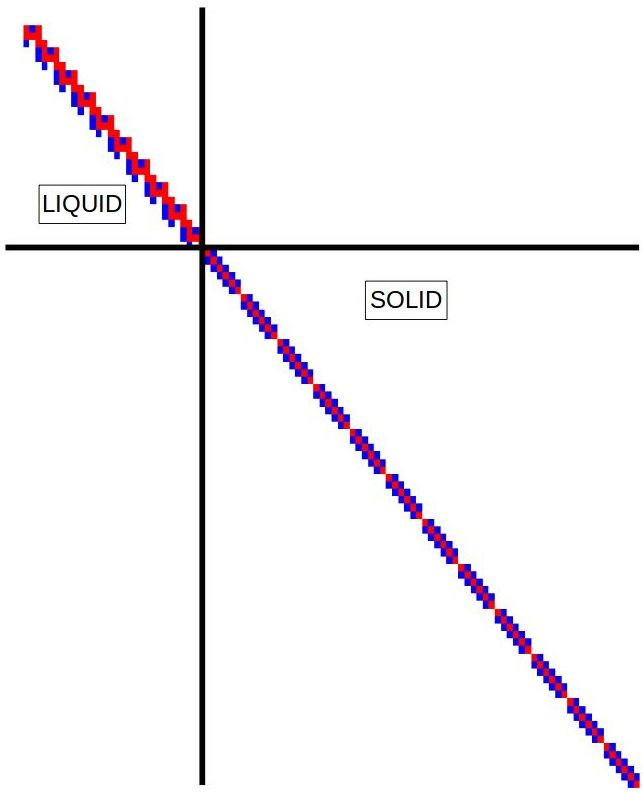
\includegraphics[width=0.40\textwidth]{images/Explicit-Diagram.jpg}
    	\caption{Strucutre of jacobian matrix for single phase liquid
    	explicitly coupled to solid conduction}
    	\label{fig:Explicit-Diagram}
    \end{figure}
    
    \begin{figure}[!h]
    	\centering
    	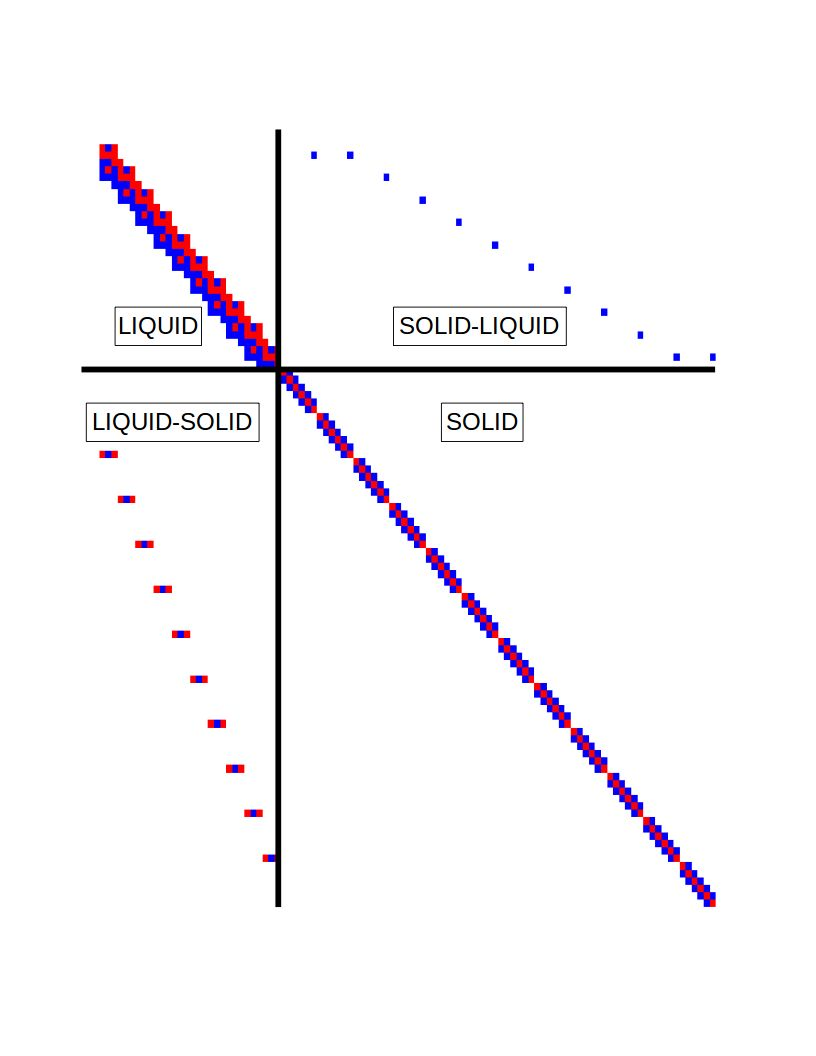
\includegraphics[width=0.40\textwidth]{images/Implicit-Diagram.jpg}
    	\caption{Strucutre of the jacobian matrix for single phase liquid
    	implicitly coupled to solid conduction}
    	\label{fig:Implicit-Diagram}
    \end{figure}
    
    Numerically building the matrix in this fashion can be very computationally
    expensive. An easy way to optimize the construction of the matrix, is to not
    compute the indexes which are known to be zero. An optional optimization
    flag was added to the code that allows for the non-zero structure to be
    remebered after the first construction, and following constructions only
    compute entries that were previously non-zero. This drastically decreases
    computations cost, but at the risk of serious potential error in the event
    of previously zero entries becoming non-zero later in the problem. For the
    verification problems covered in this work, this does not occur and
    therefore this optimization method is appropriate. Other optimization work
    could be in the parallelization of the construction and solution of the
    Jacobian matrix. 
   
    
    
    
    







%SourceDoc ../YourName-Dissertation.tex
\vspace*{-80mm}
\chapter{Isokinetic Step Advection} \label{chapter4:Isokinetic_Step_Advection}
 
	\section{Problem Setup} \label{Verification:Advection}
    
    A tube with no gravity acting in the direction of fluid flow has an initial
    condition of $U_{1},\rho_{1},h_{1},P_{1},\dot{m}_{1}$ everywhere except at the 
    starting position that has an intitial conditions of $h_{2},\rho_{2},\dot{m}_{2}$. 
    When the time step for the calcuation is taken be exactly equal to the CFL
    number as seen in equation \ref{eq:CFL}, the inlet conditions should advect
    through the rest of the system in the form of a square wave. This is a
    unique situation where the CFL can be held constant throughout the
    simulation, and where the spatial and temporal trucation error can cancel
    each other out at $CFL=1$. When the CFL is less than 1, numerical
    diffusion occurs based on the truncation terms produced by the modified
    equation analysis.
    
    \begin{equation}
    	\label{eq:CFL}
    	CFL = \frac{\Delta t  U_{0} }{\Delta x}
    \end{equation}
    
    \begin{figure}[!h]
    	\centering
    	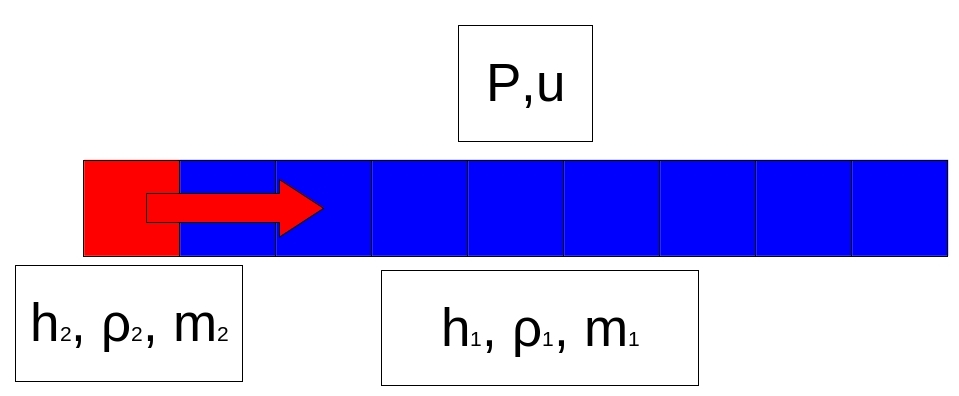
\includegraphics[width=0.65\textwidth]{images/Verification_Problem1_advection}
    	\label{fig:Verification_1}
    	\caption{Setup for the isokinetic advection problem}
    \end{figure}
    
    The problem was set up using the parameters given in table
    \ref{table:Advection_Params}. Initial temperature, density, and mass flow
    rate of the sysmte differs from the inlet temperature, density, and mass
    flow rate. The pressure and velocity of the system remains constant. The
    transient runs until the center of the advected wave reaches the end of the
    tube at roughly 60 seconds. The value of the parameters are more or less
    arbitrary, but approximate a single channel about the length of a fuel
    assembly undergoing a 10 C temperature difference. The water is close to
    standard temperature and pressure. 
    
    \begin{table}[!h]
    	\center
    	\label{table:Advection_Params}
    	\caption{Input Parameters for Isokinetic Advection}
    	\begin{tabular}{|c|c|c|}
    		\hline
	    	Length 	  				&  3.00		& m 		\\ \hline 
	    	Channel Area			&  0.0001	& $m^{2}$	\\ \hline
	    	Wetted Perimeter		&  0.040	& m			\\ \hline
	    	Pressure  				&  1.00		& bar		\\ \hline
	    	Initial Temperature		&  40.00	& C			\\ \hline
	    	Inlet Temperature		&  30.00 	& C			\\ \hline
	    	Inlet Mass Flow Rate 	&  0.005	& kg/s		\\ \hline 
	    	Inlet Density			&  992.61	& kg/$m^{3}$\\ \hline
	    	Velocity				&  0.050372	& m/s		\\ \hline
    	\end{tabular}
    \end{table}
    
    \section{Density Advection and Error}
    
    Figure \ref{fig:enthalpy_wave} compares the analytical and numerical
    advection of density through the domain for a CFL number of 0.500. The
    higher density in the colder region is on the left, and the lower density of
    the warmer region is on the right. The red line on the right of the figure
    depicts the truncation error at the current time step. The truncation error
    occurs around the original dicontinuity as it advects through the solution.
    As the discontinuity propogates it becomes more diffuse spatially. Once it
    reaches the outlet the discontiuty leaves the domain and the overall error
    drops to nearly zero. For this problem, the truncation error can be shown to
    be a direct function of the CFL number and can be reduced to nearly zero
    throughout the simulation. This simplified problem with an exact solution is
    used for code verification.
    
    \begin{figure}[!h]
    	\centering
   		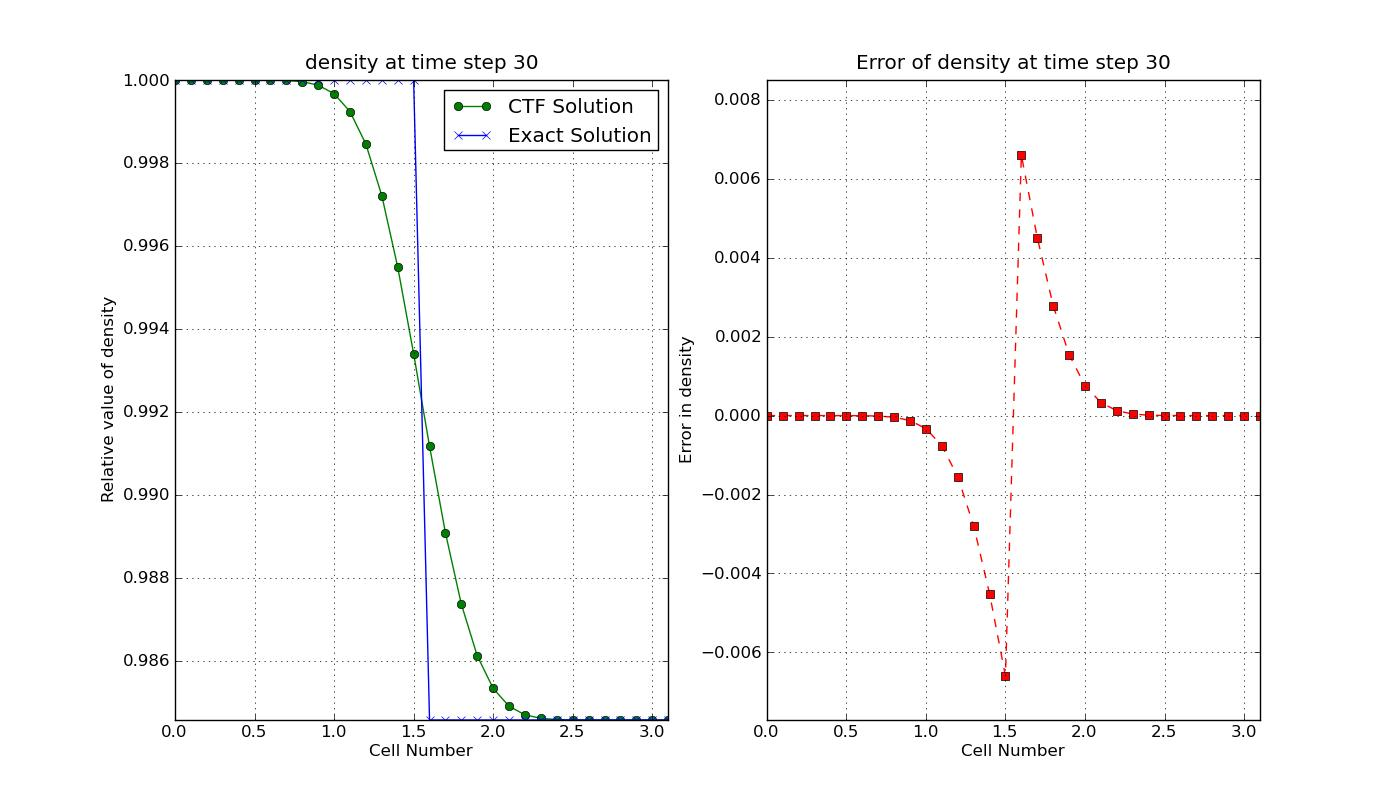
\includegraphics[width=0.85\textwidth]{images/linear_CTF_CFL_0.500/tmp/plot_density_0030}
    	\caption{Comparison of density advection to analytical solution}
    	\label{fig:enthalpy_wave}
    \end{figure}
    
    \section{Modified Equation Analysis}
    
    For this isokinetic problem, the original mass balance equation can be re-written to 
    look like equation \ref{eq:isokinetic_start}. Using upwinding, the finite difference
    can be written to look like equation \ref{eq:mass_isok_fd}. A second order Taylor 
    series approximation can be used for $\rho_{i}^{n+1}$ and $\rho_{i-1}^{n}$ as shown 
    in equations \ref{eq:rho_taylor_series_time} and \ref{eq:rho_taylor_series_space} 
    respectively. The higher order terms ($O(\Delta x^{2},\Delta t^{2} )$) are
    not taken into account for this approximation. The Taylor series
    approximations can then be substituted into \ref{eq:mass_isok_fd} to yield
    \ref{eq:MEA_start}. This is the beginning of the modified equation analysis.
    The goal will be to isolate the original PDE and define the truncation error.
    
    \begin{equation}
    	\label{eq:isokinetic_start}
    	\frac{\partial \rho}{\partial t} + U_{0} \frac{\partial \rho}{\partial x} = 0
    \end{equation}
    
    \begin{equation}
    	\label{eq:mass_isok_fd}
    	\frac{ \rho_{i}^{n+1} - \rho_{i}^{n} }{\Delta t} 
    	+ U_{0} \frac{\rho_{i}^{n} - \rho_{i-1}^{n}}{\Delta x} = 0
    \end{equation}
    
    \begin{equation}
    	\label{eq:rho_taylor_series_time}
    	\rho_{i}^{n+1} =  \rho_{i}^{n} + 
    	\frac{\partial \rho}{\partial t} \Delta t +
    	\frac{1}{2} \frac{\partial^2 \rho}{\partial t^2} \Delta t^2 + O(\Delta t^{3})
    \end{equation}
    
    \begin{equation}
    	\label{eq:rho_taylor_series_space}
    	\rho_{i-1}^{n} =  \rho_{i}^{n} - 
    	\frac{\partial \rho}{\partial x} \Delta x +
    	\frac{1}{2} \frac{\partial^2 \rho}{\partial x^2} \Delta x^2 + O(\Delta x^{3})
    \end{equation}
    
    The lengthy equation \ref{eq:MEA_start} can be reduced to equation
    \ref{eq:MEA_p0} since the $\rho_{i}^{n}$ terms subtract out and the $\Delta
    t$ and $\Delta x$ terms in the denominator cancel out. This reduced equation
    can the be re-written into equation \ref{eq:MEA_p1}, with the original PDE
    followed by the truncation terms. Notice how the terms on the right are
    dependent on both the numerical spacing $\Delta t$ and $\Delta x$, but also
    on the second derivatives of density with respect to space and time.
    
    \begin{equation}
    	\label{eq:MEA_start}
    	\frac{ \left( \rho_{i}^{n} + \frac{\partial \rho}{\partial t} \Delta t +
    	\frac{1}{2} \frac{\partial^2 \rho}{\partial t^2} \Delta t^2 \right)-\rho_{i}^{n} }{\Delta t} 
    	+ U_{0} \frac{\rho_{i}^{n} - \left( \rho_{i}^{n} -  \frac{\partial \rho}{\partial x} \Delta x + 
    	\frac{1}{2} \frac{\partial^2 \rho}{\partial x^2} \Delta x^2 \right)}{\Delta x} 
    	+ O(\Delta x^{2},\Delta t^{2}) 
    	= 0
    \end{equation}
    
    \begin{equation}
    	\label{eq:MEA_p0}
    	 \frac{\partial \rho}{\partial t}  + \frac{1}{2} \frac{\partial^2 \rho}{\partial t^2} \Delta t +
    	 U_{0} \left(   \frac{\partial \rho}{\partial x}  - \frac{1}{2} \frac{\partial^2 \rho}{\partial x^2} \Delta x \right) 
    	 + O(\Delta x^{2},\Delta t^{2}) 
    	 = 0
    \end{equation}
    
    \begin{equation}
    	\label{eq:MEA_p1}
    	 \frac{\partial \rho}{\partial t}  +  U_{0} \frac{\partial \rho}{\partial x} + 
    	 \frac{1}{2} \frac{\partial^2 \rho}{\partial t^2} \Delta t -
    	   U_{0}  \frac{1}{2} \frac{\partial^2 \rho}{\partial x^2} \Delta x  
    	   + O(\Delta x^{2},\Delta t^{2}) = 0 
    \end{equation} \linebreak
    
    Before we can procede, we need to take the derivative of the original PDE with respect
    to space and time as shown in equations \ref{eq:mass_dt} and  \ref{eq:mass_dx} 
    respectively. These two derivatives can substitute into each other using the common 
    term $\frac{\partial^2 \rho}{\partial x \partial t}$. The second derivatives of density with 
    respect to space and time are therefore related by the velocity squared as
    shown by equation \ref{eq:mass_second_derivatives}.
    
    \begin{equation}
    \label{eq:mass_dt}
    	 \frac{\partial^2 \rho}{\partial t^2} + U_{0} \frac{\partial^2 \rho}{\partial x \partial t} = 0
    \end{equation}
    
    \begin{equation}
    \label{eq:mass_dx}
    	 \frac{\partial^2 \rho}{\partial t \partial x} + U_{0} \frac{\partial^2 \rho}{\partial x^2} = 0
    \end{equation}
    
    \begin{equation}
    \label{eq:mass_second_derivatives}
    	 \frac{\partial^2 \rho}{\partial t^2} =  U_{0}^2 \frac{\partial^2 \rho}{\partial x^2}
    \end{equation} \linebreak
    
    This relationship can then be substituted back into equation \ref{eq:MEA_p1}, 
    which can be reduced to equation \ref{eq:MEA_result} after ignoring the higher
    order terms. The error depends on the CFL number, the axial spacing, and the
    second order derivative of density with respect to space. This derivative is
    what gives the error the characteristics of diffusion. When the CFL number
    is less than one, the error term is negative and the diffusion is dampening. When
    the CFL number is greater than one, the error term becomes positive, and the
    accumulation of the error destabilizes the solution. 
    
    \begin{equation}
    	 \frac{\partial \rho}{\partial t}  +  U_{0} \frac{\partial \rho}{\partial x} - 
    	  \frac{1}{2}  \left(  \Delta x U_{0} \frac{\partial^2 \rho}{\partial
    	  x^2} -   U_{0}^2 \frac{\partial^2 \rho}{\partial x^2} \Delta t  \right) 
    	   + O(\Delta x^{2},\Delta t^{2}) = 0
    \end{equation}
    
    \begin{equation}
    \label{eq:MEA_result}
    	 \frac{\partial \rho}{\partial t}  +  U_{0} \frac{\partial \rho}{\partial x} - 
    	 \frac{\Delta x U_{0}}{2} \frac{\partial^2 \rho}{\partial x^2}  
    	 \left(  1 - CFL  \right) 
    	 + O(\Delta x^{2},\Delta t^{2})  = 0
    \end{equation}
    
    Modified equation analysis can be applied to the energy balance equation
    presented in equation \ref{eq:MEA_energy}. The energy equation is presented in a form where
    the momentum equation was substituted in as zero and then divided through by
    density. The result presented in equation \ref{eq:MEA_ene_result} is similar in
    form to the result for the mass balance equation \ref{eq:MEA_result}.
    
    \begin{equation}
    	\label{eq:MEA_energy}
    	\frac{\partial h}{\partial t} - \frac{1}{\rho} \frac{\partial P}{\partial t} +
    	U_{0} \frac{\partial h}{\partial x} = 0
    \end{equation}
    
    \begin{equation}
    \label{eq:MEA_ene_result}
    	\frac{\partial h}{\partial t} - \frac{1}{\rho} \frac{\partial P}{\partial t} +
    	U_{0} \frac{\partial h}{\partial x} - 
    	\frac{\Delta x U_{0}}{2} \frac{\partial^2 h}{\partial x^2}
    	\left( 1 - CFL \right)
    	= 0
    \end{equation}
    
    \section{Scaling of Error}

	From the modified equation analysis, the advection problem should prove to
	be first order accurate in time and space. Assuming a fixed number of points,
	the time step was halved several times. The relative difference between each
	step was taken and $\ell 1$ normalized across space at at a particular time.
	The plot of this difference can be seen for density in figure
	\ref{fig:Difference_rho}. 
    
%    \begin{figure}[!h]
%    	\centering
%    	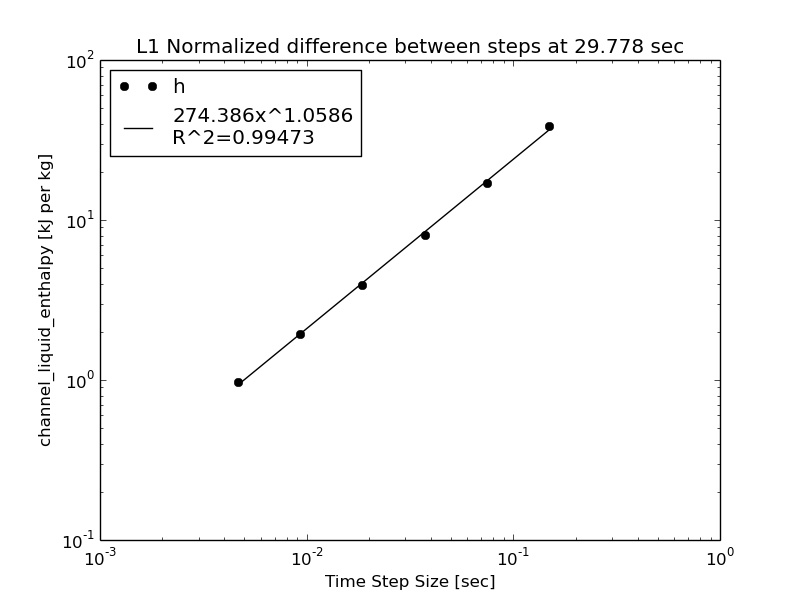
\includegraphics[width=0.50\textwidth]{images/Isokinetic_Advection/Difference_h}
%    	\caption{Scaling of numerical error with constant time step size for
%    	enthalpy}
%    	\label{fig:Difference_h}
%    \end{figure}
    
    
    \begin{figure}[!h]
    	\centering
    	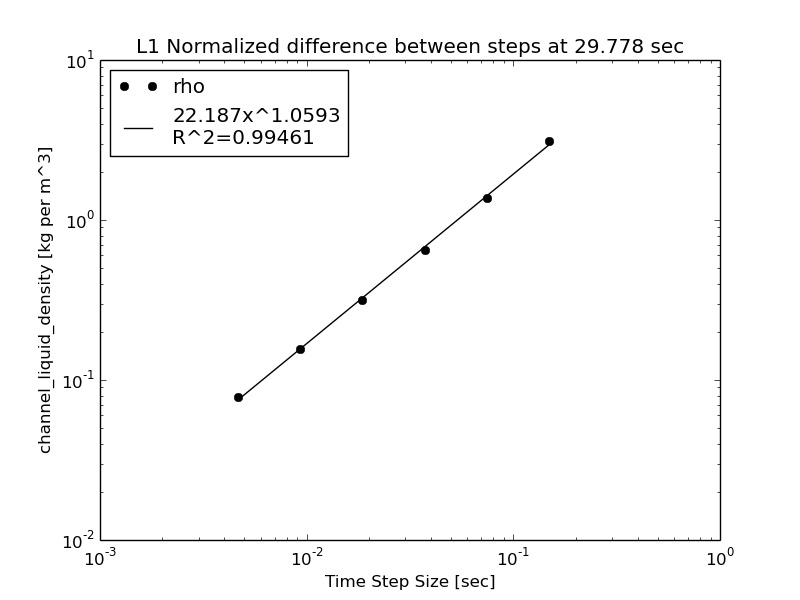
\includegraphics[width=0.60\textwidth]{images/Isokinetic_Advection/Difference_rho}
    	\caption{Scaling of numerical error with constant time step size for
    	density}
    	\label{fig:Difference_rho}
    \end{figure}
    
    The power fit for density has a high correlation coefficient, and
    shows that the order of accuracy temporally is close to 1. Richardson
    extrapolation to determine the order of accuracy at each point as shown by 
    figure \ref{fig:Temporal_Order_Of_Accuracy_rho}. As the time step size
    decreases, the order of accuracy approaches 1.0 due to smaller higher order
    terms. 
        
%   \begin{figure}[!h]
%   	\centering
%   	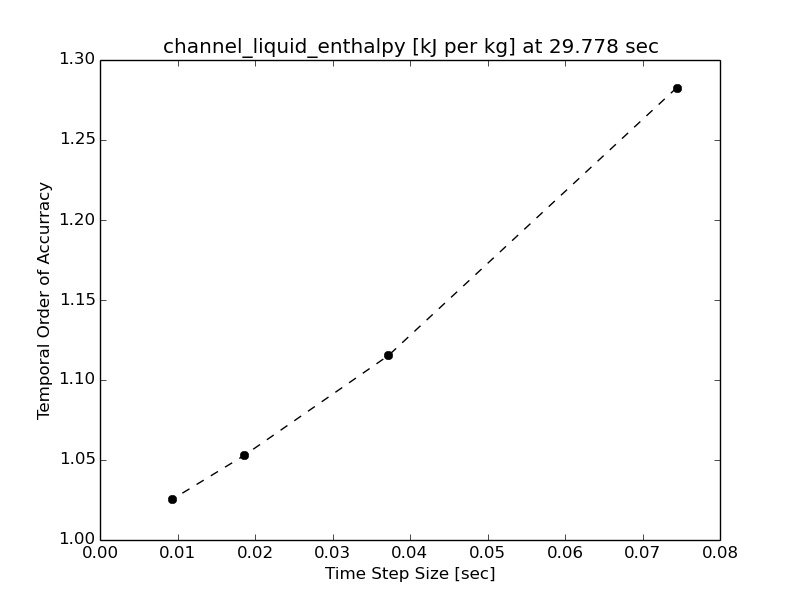
\includegraphics[width=0.50\textwidth]{images/Isokinetic_Advection/Temoral_Order_Of_Accuracy_h}
%   	\caption{Temporal Order of Accuracy for density}
%   	\label{fig:Temporal_Order_Of_Accuracy_h}
%   \end{figure}
    
    \begin{figure}[!h]
    	\centering
    	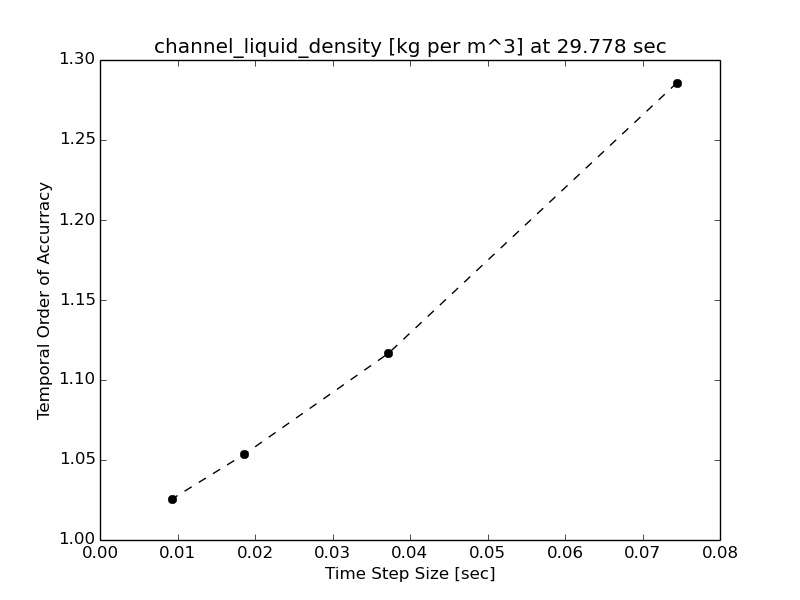
\includegraphics[width=0.60\textwidth]{images/Isokinetic_Advection/Temoral_Order_Of_Accuracy_rho}
    	\caption{Temporal Order of Accuracy for density}
    	\label{fig:Temporal_Order_Of_Accuracy_rho}
    \end{figure}
    
    When the CFL number is set to 1, the spatial error and temporal error
    cancel out producing a perfect square wave in time and space as shown by
    figure \ref{fig:density_2D}. This holds true for a variety of spatial
    mesh sizes, confirming that both the temporal and spatial errors are first
    order accurate. 
    
    \begin{figure}[!h]
    	\centering
    	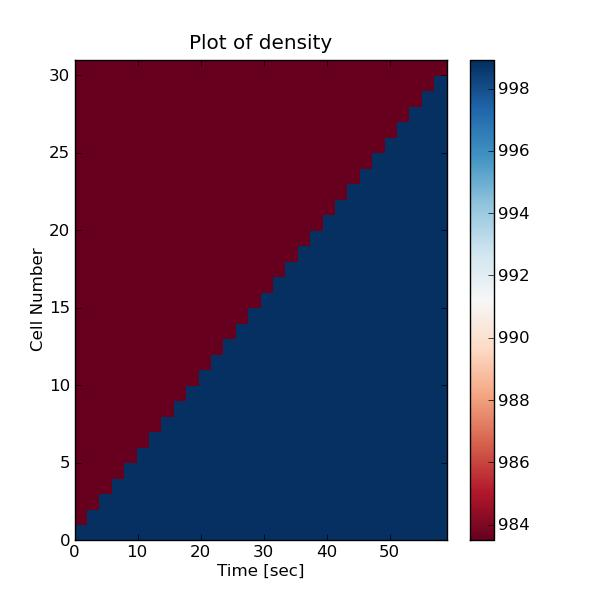
\includegraphics[width=0.60\textwidth]{images/Isokinetic_Advection/density_2D}
    	\caption{Advection of isokinetic density wave $\frac{kg}{m^{3}}$ in time
    	and space for CFL=1}
    	\label{fig:density_2D}
    \end{figure}









%%%%%%%%%%%%%%%%%%%%%%%%%%%%%%%%%%%%%%%%%%%%%%%%%%%%%%%%%%%%%%%
% Appendices
%
% Because of a quirk in LaTeX (see p. 48 of The LaTeX
% Companion, 2e), you cannot use \include along with
% \addtocontents if you want things to appear the proper
% sequence.
%%%%%%%%%%%%%%%%%%%%%%%%%%%%%%%%%%%%%%%%%%%%%%%%%%%%%%%%%%%%%%%
\appendix
\titleformat{\chapter}[display]{\fontsize{30}{30}\selectfont\bfseries\sffamily}{Appendix \thechapter\textcolor{gray75}{\raisebox{3pt}{|}}}{0pt}{}{}
% If you have a single appendix, then to prevent LaTeX from
% calling it ``Appendix A'', you should uncomment the following two
% lines that redefine the \thechapter and \thesection:
%\renewcommand\thechapter{}
%\renewcommand\thesection{\arabic{section}}
%\Appendix{Title of the First Appendix}

\section{Introduction}
When in the Course of human events, it becomes necessary for one people  to dissolve the political bands which have connected them with another,  and to assume among the powers of the earth, the separate and equal station  to which the Laws of Nature and of Nature's God entitle them, a decent respect to the opinions of mankind requires that they should declare  the causes which impel them to the separation.

\section{More Declaration}

We hold these truths to be self-evident, that all men are created equal,  that they are endowed by their Creator with certain unalienable Rights,  that among these are Life, Liberty and the pursuit of Happiness. --That to secure these  rights, Governments are instituted among Men, deriving their just powers  from the consent of the governed, --That whenever any Form of Government  becomes destructive of these ends, it is the Right of the People to alter  or to abolish it, and to institute new Government, laying its foundation on  such principles and organizing its powers in such form, as to them shall  seem most likely to effect their Safety and Happiness.

\subsection{Some Subsection Title Here}

Prudence, indeed, will dictate that Governments long established should not  be changed for light and transient causes; and accordingly all experience  hath shewn, that mankind are more disposed to suffer, while evils are  sufferable, than to right themselves by abolishing the forms to which they  are accustomed. But when a long train of abuses and usurpations, pursuing invariably the same  Object evinces a design to reduce them under absolute Despotism, it is their  right, it is their duty, to throw off such Government, and to provide new Guards for their future security. --Such has been the patient sufferance of these Colonies; and such is now the  necessity which constrains them to alter their former Systems of Government.  The history of the present King of Great Britain [George III] is a history  of repeated injuries and usurpations, all having in direct object the  establishment of an absolute Tyranny over these States. To prove this, let Facts be submitted to a candid world.
%\Appendix{Title of the Fifth Appendix}

\section{Introduction}
When in the Course of human events, it becomes necessary for one people  to dissolve the political bands which have connected them with another,  and to assume among the powers of the earth, the separate and equal station  to which the Laws of Nature and of Nature's God entitle them, a decent respect to the opinions of mankind requires that they should declare  the causes which impel them to the separation.

\pagebreak
Some text.
{\lstset{language=Fortran}
\footnotesize
\begin{lstlisting}
      program chaos
c When a LS Fortran program has been compiled and linked into Mac
c application, all information written to the screen WRITE(6,...) or
c WRITE(*,...) appears in a standard Mac window, complete with basic
c menus.
      external fex, jac
      double precision atol, rtol, rwork, t, tout, h
      double precision ttotal, dtout
      dimension h(3), atol(3), rwork(70), iwork(23)
	  character*8 tstart, tend
      neq = 3
	  
	  call time(tstart)
	  write(6,*) "begin integration at  ", tstart
      write(6,*)
	  
c --- Read in the total initial angular momentum.  The total angular
c     momentum H is always unity due to normalization.
	  open(unit = 2, file = 'chaos.data', status = 'unknown')
      read(2,*) h(1), h(2), h(3)
	  
c --- The integration begins at t = 0 and the values are printed at
c     every tout.  tout is incremented below.  ttotal is the length
c     of the entire integration.  The number of recorded values of
c     the integration is given by npoints.
      t = 0.0d0
      tout = 0.0d0
      write(6,*) 'Duration of integration interval, i.e., tfinal?'
      read(6,*) ttotal
      write(6,*)
      write(6,*) 'Number of points for trajectory plot?'
      read(6,*) npoints
      write(6,*)
      dtout = ttotal/dfloat(npoints)
      tout = tout + dtout
	  
c --- Tolerance parameters used by lsoda.
      itol = 2
      rtol = 1.0d-9
      atol(1) = 1.0d-9
      atol(2) = 1.0d-9
      atol(3) = 1.0d-9
	  
c --- Other parameters used by lsoda.  See below.
      itask = 1
      istate = 1
      iopt = 1
      lrw = 70
      liw = 23
      jt = 1

      do 11 kount = 5,10
         rwork(kount) = 0.0d0
         iwork(kount) = 0
  11  continue
      iwork(6) = 100000
	  
	  open(unit = 3, file = 'traj.dat', disp = 'keep',
     &     status = 'unknown')
	 
c --- The actual integration begins here.  Loop on the value of iout.
      do 40 iout = 1, npoints
	  
         call lsoda(fex,neq,h,t,tout,itol,rtol,atol,itask,istate,
     &              iopt,rwork,lrw,iwork,liw,jdum,jt)
	  
c ------ Write the output to the file traj.dat.
         write(3,20) t, h(1), h(2), h(3)
  20     format(f9.1, 3e15.6)

         if (mod(tout,5000.0d0) .eq. 0.0d0) then
            write(6,*) tout
         end if
  
c ------ Check to see that things are going OK.
         if (istate .lt. 0) go to 80
		 
c ------ Set the time at which the integration is next recorded and
c        continue the do-loop.
  40     tout = tout + dtout
  
      write(6,*) 'number of steps taken: ', iwork(11)
      write(6,*) 'number of f evaluations: ', iwork(12)
      write(6,*) 'number of Jacobian evaluations: ', iwork(13)
      write(6,*) 'method order last used: ', iwork(14)
      write(6,*) 'method last used (2 = stiff): ', iwork(19)
      write(6,*) 'value of t at last method switch: ', rwork(15)
      write(6,*)
	 
	  call time(tend)
	  write(6,*) "end integration at  ", tend
      stop
	  
c --- If there is an error, given by istate < 0, write the following.
  80  write(6,90) istate
  90  format(///22h error halt.. istate =,i3)
  
      stop
      end

\end{lstlisting}
}

%%%%%%%%%%%%%%%%%%%%%%%%%%%%%%%%%%%%%%%%%%%%%%%%%%%%%%%%%%%%%%%
% ESM students need to include a Nontechnical Abstract as the %
% last appendix.                                              %
%%%%%%%%%%%%%%%%%%%%%%%%%%%%%%%%%%%%%%%%%%%%%%%%%%%%%%%%%%%%%%%
% This \include command should point to the file containing
% that abstract.
%\include{nontechnical-abstract}
%%%%%%%%%%%%%%%%%%%%%%%%%%%%%%%%%%%%%%%%%%%
} % End of the \allowdisplaybreak command %
%%%%%%%%%%%%%%%%%%%%%%%%%%%%%%%%%%%%%%%%%%%

%%%%%%%%%%%%%%%%
% BIBLIOGRAPHY %
%%%%%%%%%%%%%%%%
% You can use BibTeX or other bibliography facility for your
% bibliography. LaTeX's standard stuff is shown below. If you
% bibtex, then this section should look something like:
	\begin{singlespace}
	\bibliographystyle{GLG-bibstyle}
	\addcontentsline{toc}{chapter}{Bibliography}
	\bibliography{CADances-thesis}
	\end{singlespace}

%\begin{singlespace}
%\begin{thebibliography}{99}
%\addcontentsline{toc}{chapter}{Bibliography}
%\frenchspacing

%\bibitem{Wisdom87} J. Wisdom, ``Rotational Dynamics of Irregularly Shaped Natural Satellites,'' \emph{The Astronomical Journal}, Vol.~94, No.~5, 1987  pp. 1350--1360.

%\bibitem{G&H83} J. Guckenheimer and P. Holmes, \emph{Nonlinear Oscillations, Dynamical Systems, and Bifurcations of Vector Fields}, Springer-Verlag, New York, 1983.

%\end{thebibliography}
%\end{singlespace}

%\backmatter

% Vita
%\vita{SupplementaryMaterial/Vita}

\end{document}

